\documentclass{InsightArticle}

\usepackage[dvips]{graphicx}
\usepackage{float}
\usepackage{subfigure}

\usepackage[dvips,
bookmarks,
bookmarksopen,
backref,
colorlinks,linkcolor={blue},citecolor={blue},urlcolor={blue},
]{hyperref}

\title{Clustering Segmentation for VTK}

% 
% NOTE: This is the last number of the "handle" URL that 
% The Insight Journal assigns to your paper as part of the
% submission process. Please replace the number "1338" with
% the actual handle number that you get assigned.
%
\newcommand{\IJhandlerIDnumber}{3309}

% Increment the release number whenever significant changes are made.
% The author and/or editor can define 'significant' however they like.
\release{0.00}

% At minimum, give your name and an email address.  You can include a
% snail-mail address if you like.

\author{David Doria}
\authoraddress{Rensselaer Polytechnic Institute}


\begin{document}

\IJhandlefooter{\IJhandlerIDnumber}


\ifpdf
\else
   %
   % Commands for including Graphics when using latex
   % 
   \DeclareGraphicsExtensions{.eps,.jpg,.gif,.tiff,.bmp,.png}
   \DeclareGraphicsRule{.jpg}{eps}{.jpg.bb}{`convert #1 eps:-}
   \DeclareGraphicsRule{.gif}{eps}{.gif.bb}{`convert #1 eps:-}
   \DeclareGraphicsRule{.tiff}{eps}{.tiff.bb}{`convert #1 eps:-}
   \DeclareGraphicsRule{.bmp}{eps}{.bmp.bb}{`convert #1 eps:-}
   \DeclareGraphicsRule{.png}{eps}{.png.bb}{`convert #1 eps:-}
\fi


\maketitle


\ifhtml
\chapter*{Front Matter\label{front}}
\fi

\begin{abstract}
\noindent

This document presents a VTK implementation of the algorithm described in 
"A clustering method for efficient segmentation of 3D laser data" by Klasing, Klaas Wollherr, Dirk, and Buss, Martin. The algorithm .

The code is available here:
\verb|https://github.com/daviddoria/ClusteringSegmentation|

\end{abstract}

\IJhandlenote{\IJhandlerIDnumber}

\tableofcontents
%%%%%%%%%%%%%%%%%%%%
\section{Introduction}
This document presents a VTK implementation of an algorithm to find clusters in a point cloud. It implicitly uses a Radially Bounded Nearest Neighbor (RBNN) graph. This implementation is based on \cite{klasing}.

%%%%%%%%%%%%%%%%%%%%
\section{Algorithm}
\label{sec:Algorithm}
\begin{itemize}
 \item Iterate over all points. For each point:
   \begin{itemize}
    \item If the point already belongs to a cluster, skip it.
    \item Find all neighbors within distance $r$.
    \item If any of these neighbors is already in a cluster, assign the current point to the same cluster, then assign all neighbors without a cluster to the same cluster.
    \item If the current point has been assigned to a cluster and there exist neighbors assigned to different clusters, merge all these clusters.
  \end{itemize}
\end{itemize}

In this implementation, the cluster that each point belongs to is stored in a vtkPointData array of the output vtkPolyData called ``ClusterID''.

%%%%%%%%%%%%%%%%%%%%
\section{Parameters}
The only parameter to the algorithm is the radius of the nearest neighbor lookup. We provide a flag ``UseAutoRadius'' that attempts to select a reasonable radius for the nearest neighbor lookup based on the extent of the data.

%%%%%%%%%%%%%%%%%%%%
\section{Demonstration}

A demonstration of the algorithm is shown in Figure \ref{fig:Demo}.

\begin{figure}[H]
\centering
\subfigure[Input point cloud.]
  {
  
\includegraphics[width=0.3\linewidth]{images/input}
  \label{fig:Demo:Input}
  }
\subfigure[Output point cloud.]
  {
  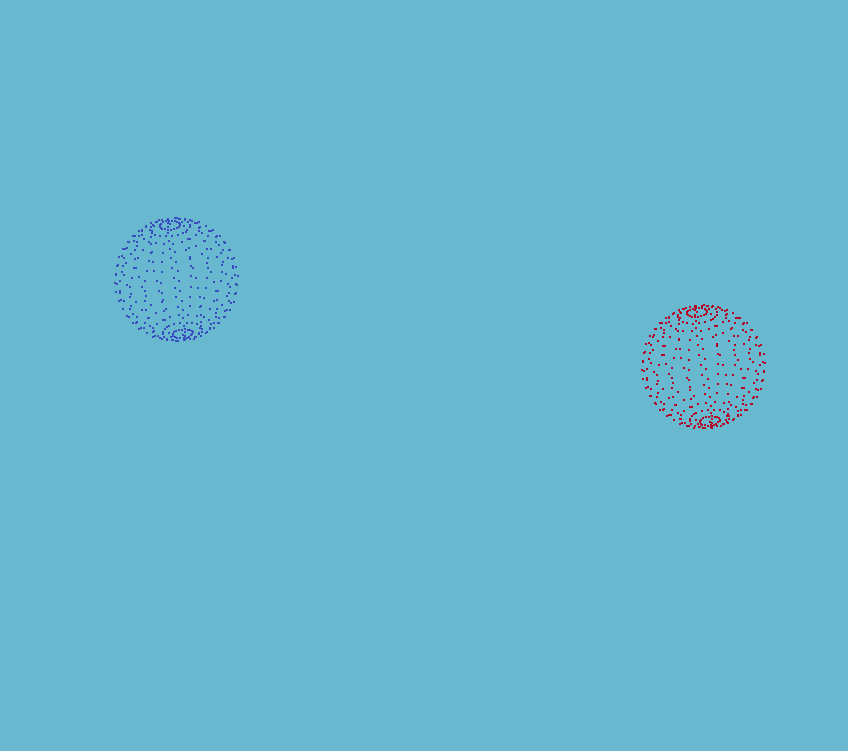
\includegraphics[width=0.3\linewidth]{images/output}
  \label{fig:Demo:Output}
  }
\caption{An example clustering.}
\label{fig:Demo}
\end{figure}

%%%%%%%%%%%%%%%%%%%%
\section{Code Snippet}
The interface to the filter is very straight forward. Simply pass it a vtkPolyData, and it will return a vtkPolyData with a new field ``ClusterID'' attached to each point.

\begin{verbatim}
  vtkSmartPointer<vtkXMLPolyDataReader> reader = 
    vtkSmartPointer<vtkXMLPolyDataReader>::New();
  reader->SetFileName(inputFileName.c_str());
  reader->Update();

  vtkSmartPointer<vtkClusteringSegmentation> clusteringSegmentation =
    vtkSmartPointer<vtkClusteringSegmentation>::New();
  clusteringSegmentation->SetInputConnection(reader->GetOutputPort());
  clusteringSegmentation->SetUseAutoRadius(true);
  clusteringSegmentation->Update();

  vtkSmartPointer<vtkXMLPolyDataWriter> writer =
    vtkSmartPointer<vtkXMLPolyDataWriter>::New();
  writer->SetFileName(outputFileName.c_str());
  writer->SetInputConnection(clusteringSegmentation->GetOutputPort());
  writer->Write();
\end{verbatim}

%%%%%%%%%%%%%%%%%%%%
\begin{thebibliography}{9}
	\bibitem{klasing}
	  Klasing, Klaas Wollherr, Dirk, and Buss, Martin,
	  \emph{A clustering method for efficient segmentation of 3D laser data}.
	  2008 IEEE International Conference on Robotics and Automation

\end{thebibliography}

\end{document}
